%%%%%%%%%%%%%%%%%%%%%%%%%%%%%%%%%%%%%%%%%
% Tufte Essay
% LaTeX Template
% Version 2.0 (19/1/19)
%
% This template originates from:
% http://www.LaTeXTemplates.com
%
% Authors:
% The Tufte-LaTeX Developers (https://www.ctan.org/pkg/tufte-latex)
% Vel (vel@LaTeXTemplates.com)
%
% License:
% Apache License, version 2.0
%
%%%%%%%%%%%%%%%%%%%%%%%%%%%%%%%%%%%%%%%%%

\documentclass[a4paper]{tufte-handout}
\usepackage{graphicx}
\usepackage{amsmath, amsfonts, amssymb, amsthm}
\usepackage{units}
\usepackage{booktabs}

\setkeys{Gin}{width=\linewidth, totalheight=\textheight, keepaspectratio}
\graphicspath{{Figures/}{./}}

\title{Summary of the Search Engines Source}
\author{Filippo Mazzarotto}
\date{Acadamic year 2024/25}

\begin{document}

\maketitle

%----------------------------------------------------------------------------------------
%	ABSTRACT/SUMMARY
%----------------------------------------------------------------------------------------

\begin{abstract}
	\textbf{Contents.} This document provides a comprehensive overview of Information Retrieval (IR) systems, including their design and development methodologies, various architectural alternatives, and performance evaluation techniques. It delves into the features and functioning of IR systems, with a particular focus on search engines, recommender systems, and other information access systems. The aim is to offer a detailed understanding of how these systems are constructed, how they operate, and how their effectiveness can be measured.
\end{abstract}

%----------------------------------------------------------------------------------------
%	ESSAY BODY
%----------------------------------------------------------------------------------------

\section{Introduction to Information Retrieval}\label{sec:introduction-to-search-engines}

By Information Retrival (IR) we mean the task of finding resources relevant to a specific need, specifed in some query. This is a fundamental task and it's been driving the development of new technology for decades. These include parallel computing, distributed systems, machine learning, natural language processing, big data comptuing, to say a few.

\begin{quote}
	''Information Retrival (IR) is a field concerned with the structure, analysis, organization, storage, searching, and retrieval of information.'' --- Gerard Stalton, 1968\cite{Salton1968}
\end{quote}

By resources we usually mean any type of text media, generally referred as "document". They may or may not have some type of structure to them. 

The IR process can be divided into three main steps: indexing, searching, and ranking.

Ranking is a multi-step process that involves Retrival, Ranking, ReRanking, reducing the magnitude of the results from $10^9$ to $10^6$ to $10^3$ to around $10$, the size of the first page of a search engine.

\subsection{Examples of Information Retrival Systems}

To design effective IR we need to leverage its specific use-case. Different cases have different requirements and goals, and thus need different approaches. Here are some examples:

\textbf{Web Search.} The Information Retrieval done by Search Engines makes extensive use of Natural Language Processing, ranking algorithms (supported by user interaction data), and personalization trough user history, location and preference to provide relevant results to a query which is usually short\sidenote{The average google query is about 2.7 words.} and out of context. It's not unusual for the user to refine its query, searching multipe time.

\textbf{Library Search.} The user is usually looking for a specific document, and the query is usually better defined. It may require expert knowledge to search effectively using the library taxonomy.

\textbf{Social Media Search.} The text in the body probabbly contains jargon, abbreviations, emojis, errors, and possibly a multitude of languages. This makes the search harder, but the system can leverage hashtags, tags, interactions and the user's network to better find and rank results.

\textbf{Local Search.} The user is looking for files and locations on its computer. It's usually slow and ineffective because of the high user-specificity of the structure and the impossibility of having lack of large-scale statistics.

\textbf{Mail Search.} The system can leverage the structure of the email, the sender, the receiver, etc. to provide better results.

\textbf{Product Search.} IR is used in conjunction with a database and a recommendation system\sidenote{Recommendation systems keep track of the user's preferences and suggest products that are likely to be of interest, without the need of a query.}.

\textbf{Conversational Search.} Chat-bots can't give long lists, but aims to one result per query in output, the input is also very verbose, it must keep extensive context histroy. but it can also ask back the user and use the context windows to remove ambiguity.

\textbf{Media Search.} Image and Audio. With the advent of Neural Networks and embeddings, they are now similar to text-based search.

\textbf{Legal Search.} Lawyers want all possible results with specific querys to prepare for a case, the ranking by relevance is not important. This is called "Recall task".


\subsection{The Knowledge Pyramid}

\begin{marginfigure}
	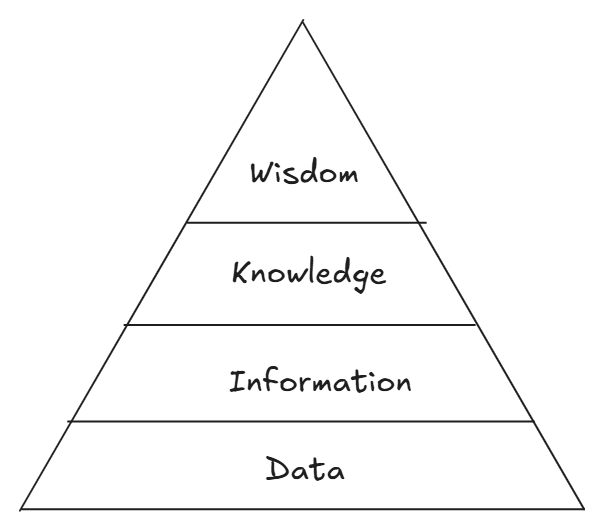
\includegraphics[width=\linewidth]{dikw-pyramid.png}
	\caption{The Knowledge Pyramid.}
	\label{fig:dikw}
\end{marginfigure}

The Knowledge Pyramid is a simplistic model for representing the hierarchy of Data, Information, Knowledge, and Wisdom. Data can be used to create information; information can be used to create knowledge, and knowledge can be used to create Wisdom.

\begin{table}[ht]
	\centering
	\fontfamily{ppl}\selectfont
	\renewcommand{\arraystretch}{1.5} % Increase the row height
	\begin{tabular}{l p{6cm}}
		\toprule
		Level & Description \\
		\midrule
		Data & Raw, unprocessed facts and figures without any context. \\
		Information & Data that is processed and organized to provide meaning. \\
		Knowledge & Information that is analyzed and understood to form insights. \\
		Wisdom & The ability to make sound decisions and judgments based on knowledge.\\
		\bottomrule
	\end{tabular}
	\caption{The Knowledge Pyramid levels and their descriptions.}
	\label{tab:knowledge-pyramid}
	\setfloatalignment{c}
\end{table}

\vspace{1em}

To retrive information, the systems needs to extract data from the documents, and then organize it. IR is not concerned with the knowledge, analysis and understaind of said information. 

\subsection{Difference between Information Retrival and Databases}

Although IR and databases both strive to retrieve information, they have diffrent specific goals and requirements, resulting in significant differences in their approaches.

\begin{quote}
	''A database is a collection of related data. By data, we mean known facts that can be recorded and that have implicit meaning. A database management system (DBMS) is a computerized system that enables users to create and maintain a database.'' --- Ramex Elmasri 2015\cite{Elmasri2015}
\end{quote}

Databases handle structured data with clear semantics based on formal models, they have well-defined attributes with certain domains that defines the possible operations. Their queries are unambiguous, and the result precise and exact.

IR systems, on the other hand, deal with mostly unstructured data, like free text, with varying levels of organization. The queries are often vague and imprecise, thus the results can't be exact. Instead IR systems aim to provide the best match through ranking, and rely on iterative, interactive processes, allowing users to refine queries based on initial results.



%----------------------------------------------------------------------------------------
%	BIBLIOGRAPHY
%----------------------------------------------------------------------------------------

\newpage

\bibliography{sample.bib}
\bibliographystyle{plainnat}

%----------------------------------------------------------------------------------------

\end{document}
